\documentclass{IEEEtran}

\usepackage[english]{babel}
\usepackage{float}

\usepackage{graphicx}
\usepackage[colorlinks=true, allcolors=blue]{hyperref}

\usepackage[letterpaper,top=2cm,bottom=2cm]{geometry}

\usepackage{listings}
\usepackage{xcolor}

\definecolor{codegreen}{rgb}{0,0.6,0}
\definecolor{codegray}{rgb}{0.5,0.5,0.5}
\definecolor{codepurple}{rgb}{0.58,0,0.82}
\definecolor{backcolour}{rgb}{0.95,0.95,0.92}

\lstdefinestyle{mystyle}{
    backgroundcolor=\color{backcolour},   
    commentstyle=\color{codegreen},
    keywordstyle=\color{magenta},
    numberstyle=\tiny\color{codegray},
    stringstyle=\color{codepurple},
    basicstyle=\ttfamily\footnotesize,
    breakatwhitespace=false,         
    breaklines=true,                 
    captionpos=b,                    
    keepspaces=true,                 
    numbers=left,                    
    numbersep=5pt,                  
    showspaces=false,                
    showstringspaces=false,
    showtabs=false,                  
    tabsize=2
}

\lstset{style=mystyle}

\date{December 13, 2024}
\title{Final Project}
\author{Terrence Jackson}

\begin{document}
\maketitle


\begin{abstract}
Is there a way to make embedded controls smarter? Controls systems are inherently rigid, based on requirements standards that implement code.  What if there was a way to have the Control System suggest better or more efficient ways to produce  a desired outcome.  What if the Control System user wasn't always correct in the input of the controls?
\end{abstract}

\section{Introduction}

By nature of the Control System architecture, the system should follow a rigid set of rules developed, architect,  and designed and documented by requirements set.  So what is expected to happen in a situation, should happen and react according to those set of standards. That is the basis of controls. 

Controls Systems have a basis where the system under control is managed in a way to perform a task and give certain outcome based on inputs that also include those controls.  Also, there is inherently a 'controller' which may be some user or set of users that react and input commands to that system.  Sometimes those controllers' inputs could be optimized.  


\section{Results}

The Chart \ref{fig:graph} below is a diagram showing how much of the inputs from outside users may affect the outcome of the Controls System given a set of inputs. These outcomes can vary greatly but may also be optimized in some cases to reduce the load and/or response time from the user. 

\begin{figure}[h]
    \centering
    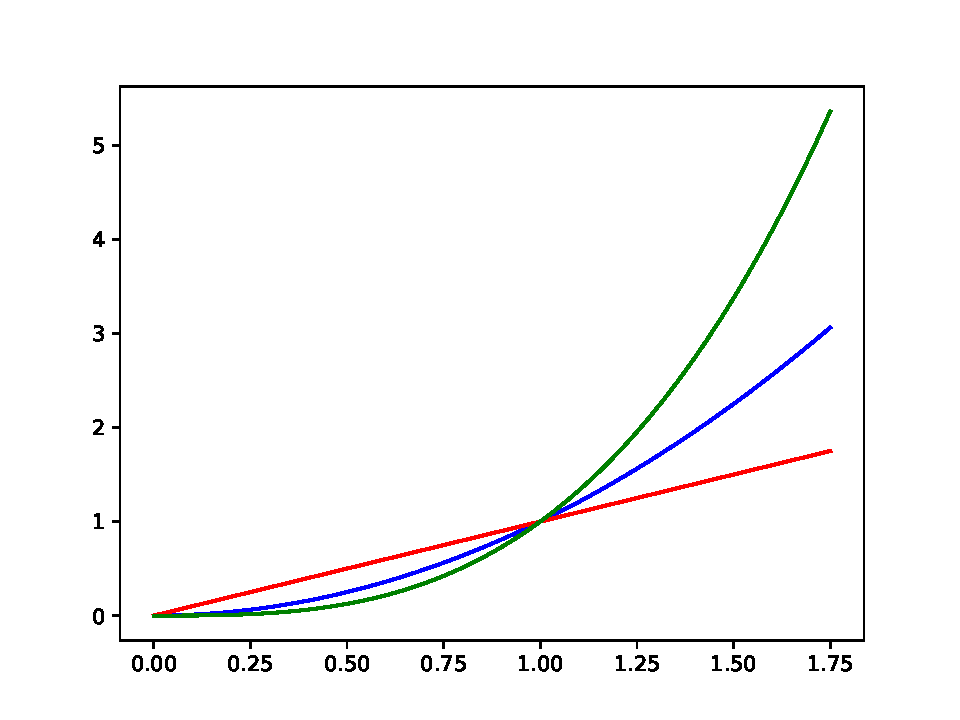
\includegraphics[width=0.65\linewidth]{Midterm_Jackson.pdf}
    \caption{\label{fig:graph} Controls Systems Chart}
\end{figure}


\section{Design}

\underline{API}

\begin{itemize}
    \item \textbf{int imul(int x, int y)}
    \newline
    This function takes in two integers and returns a the result of multiplying those integers using an iterative method.

    \item \textbf{int idiv(int n, int d)}
    \newline
    This function takes a numerator and denominator and returns the quotient of dividing the numerator n by the denominator d. The remainder is not returned.

    \item \textbf{Makefile}
    \newline
    This file contains the ruleset for running and compiling the project. Simply run 'make' and the code will compile. After that run 'X2' and the executeable file will run

    \lstinputlisting[language=bash]{MakeExample.txt}
    
\end{itemize}

\section{Conclusion}

Based on the outlined findings previously stated, it is within reason to conclude that Controls Systems can be improved in nominal/critical cases where time to react, outcomes desired, and other data factors may help to improve system efficiency and desired outcomes. 

For the Final Project the C program written using an iterative method to multiplication and division was compared to running with the multiplication and division symbols in C.  The results are displayed in Figure \ref{fig:graph2}. The iterative method takes an exponentially increasing amount of time with larger inputs.  

\begin{figure}[h]
    \centering
    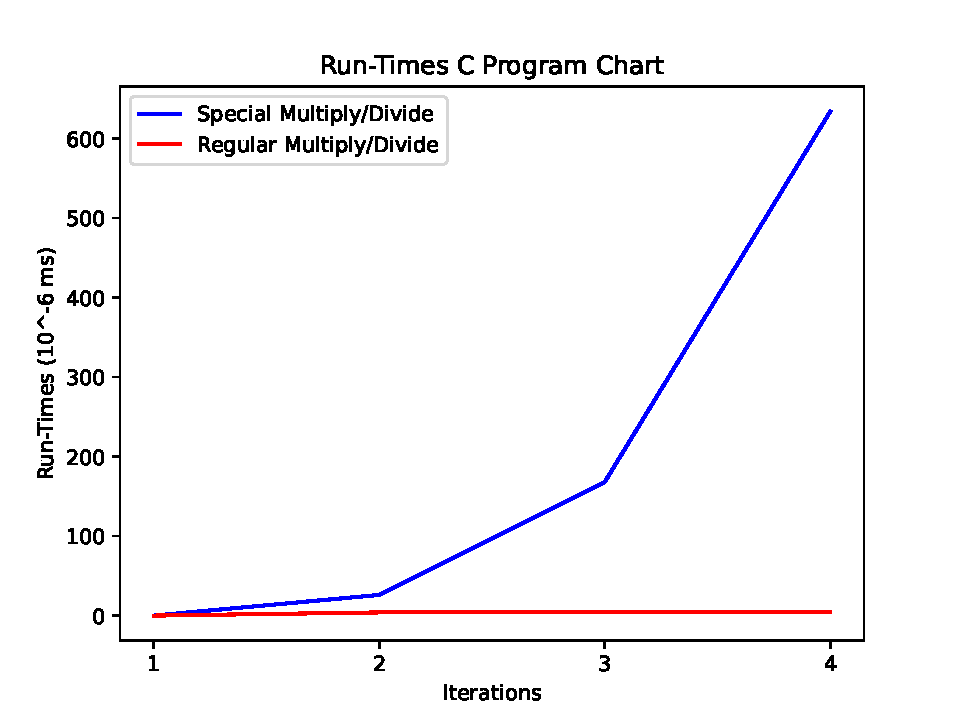
\includegraphics[width=0.65\linewidth]{ECGR5100_FinalProj.pdf}
    \caption{\label{fig:graph2} C Program Run-Times }
\end{figure}



\end{document}